\documentclass{article}
\usepackage[utf8]{inputenc}

\title{\underline{\textit{\Large{ASSIGNMENT 10: LINEAR AND CIRCULAR CONVOLUTION}}}}
\author{\textit{ SHAILESH PUPALWAR, EE20B100 }}
\date{\today}

\usepackage{natbib}
\usepackage{graphicx}
\usepackage{amsmath}
\usepackage{listings}
\usepackage{alltt}
\begin{document}

\maketitle

\section{Introduction}
In this assignment we focus on convolution. Here, we perform the convolution using 3 methods:  (i) Linear (ii) Circular and (iii) Circular using Linear convolutions. We also perform auto correlations on shifted versions of the Zadoff-Chu Sequence.

\section{Assignment questions}

\subsection{Helper Functions}
A helping function for plotting the graph has been used throughout the code.
\lstset{language=Python}
\lstset{frame=lines}
\lstset{label={lst:code_direct}}
\lstset{basicstyle=\footnotesize}
\begin{alltt}
def make_graph(xVal, yVal, xL = '\omega', yL = 'Magnitude', head = 'xyz', save = 'x.png'):
    plot(xVal, yVal)
    xlabel(xL)
    ylabel(yL)
    title(head)
    grid(True)
    savefig(save) 
\end{alltt}

\subsection{Question 1}
After downloading the "h.csv" file, we are reading the contents of it through following code snippet:- 
\begin{alltt}
file1 = "h.csv"

b = np.zeros(12)
i = 0
with open(file1, 'r') as f1:  
    for line in f1:
        b[i] = float(line) 
        i += 1
\end{alltt}
\subsection{Question 2}
We first use scipy.signal.freqz() to convert the given filter from the time domain to the frequency domain(frequency response). 
\begin{alltt}
w, h = sp.freqz(b)
figure(0)
subplot(2, 1, 1)
make_graph(w,abs(h),'','|H| (Magnitude) →', 'Q2: Magnitude and phase response 
for Low pass filter')
subplot(2, 1, 2)
make_graph(w, angle(h), '\omega →', '∠H (phase) →' , '')
savefig("Ass10_Figure_1.png"), show()
\end{alltt}
The plots obtained represent an LPF:-
\begin{figure}[h!]
\centering
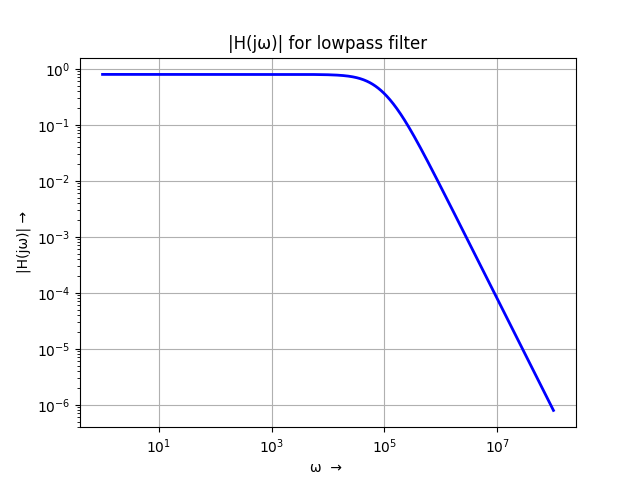
\includegraphics[scale=0.6]{Figure_0.png}
\caption{Magnitude and phase plot for LPF}
\label{fig:universe}
\end{figure}


\subsection{Question 3}
We generate the input function in this part.
\begin{alltt}
n = array(range(2**10))
x = cos(0.2*pi*n) + cos(0.85*pi*n) # Generating the signal 
make_graph(n, x, 'n →', 'x →', 'Q3: 
Plot of sequence, x = cos(0.2/u03C0n) + cos(0.85/u03C0n)', "Ass10_Figure_2.png"), show()
\end{alltt}

\begin{figure}[h!]
\centering
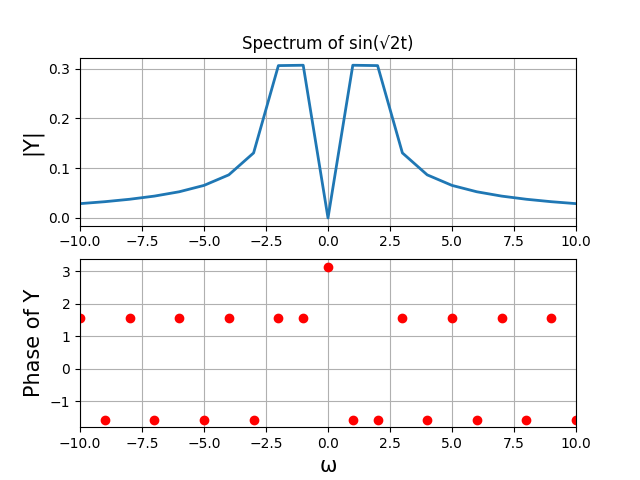
\includegraphics[scale=0.6]{Figure_1.png}
\caption{Plot of sequence x(.): $cos(0.2\pi n)+cos(0.85\pi n)$}
\label{fig:universe}
\end{figure}

\newpage
\subsection{Question 4}
We first do linear convolution using the formula :
\begin{equation}
    y[n] = \sum_{k=0}^{n-1} x[n-k]h[k]
\end{equation}
\begin{alltt}
y = np.zeros(len(x))
# Loop for convolution
for i in arange(len(x)):
    for k in arange(len(b)):
        y[i] += x[i-k]*b[k]
    
make_graph(n, y, 'n →', 'y →', 'Q4: Output of linear convolution: y(n) = x(n) * b(n)',
"Ass10_Figure_3.png"), show()
\end{alltt}

\begin{figure}[h!]
\centering
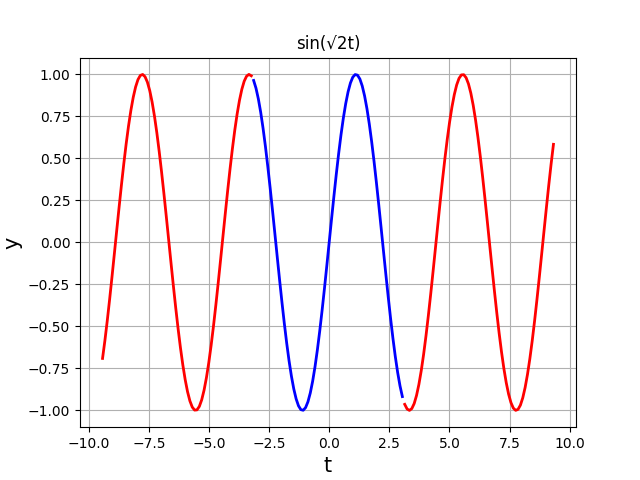
\includegraphics[scale=0.6]{Figure_2.png}
\caption{Linear Convolution of x and b}
\label{fig:universe}
\end{figure}
\clearpage

\subsection{Question 5}
We attempt to solve this more efficiently. Hence we shift to circular convolutions, where we convert to the frequency domain, multiply and go back to the time domain.
\begin{alltt}
y = ifft(fft(x)*fft(concatenate((b, zeros(len(x) - len(b))))))
make_graph(n, real(y), 'n →', 'Re{y} →', 'Q5: Output of circular convolution', 
"Ass10_Figure_4.png"), show()
\end{alltt}
\begin{figure}[h!]
\centering
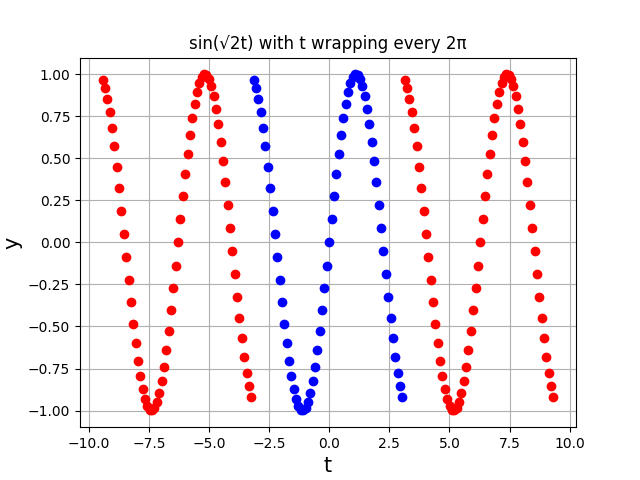
\includegraphics[scale=0.6]{Figure_3.png}
\caption{Circular Convolution of x and b}
\label{fig:universe}
\end{figure}

\subsection{Question 6}
We realize that this efficient solution is non causal and requires the entire signal to perform a convolution. We now implement a linear method of circular convolution so that we need not depend on the next infinite values in the input but only a finite number of values(this is still non causal but the delay in the response is lower)
\begin{alltt}

def circular_conv(x, h):
    P = len(h)
    n_temp = int(ceil(log2(P)))
    h_temp = np.concatenate((h, np.zeros(int(2**n_temp) - P)))
    P = len(h_temp)
    n1 = int(ceil(len(x)/2**n_temp))
    x_temp = np.concatenate((x, np.zeros(n1*(int(2**n_temp)) - len(x))))
    y = np.zeros(len(x_temp) + len(h_temp) - 1)
    for i in range(n1):
        temp = np.concatenate((x_temp[i*P:(i + 1)*P], np.zeros(P - 1)))
        y[i*P:(i + 1)*P + P - 1] += np.fft.ifft(np.fft.fft(temp) * np.fft.fft( 
        np.concatenate((h_temp,np.zeros(len(temp)-len(h_temp))) ))).real
    return y

y = circular_conv(x, b)
make_graph(n, real(y[:1024]), 'n →', 'Re{y} →', 'Q6: Output of circular convolution using 
linear convolution', "Figure_4.png"), show()

\end{alltt}
\begin{figure}[h!]
\centering
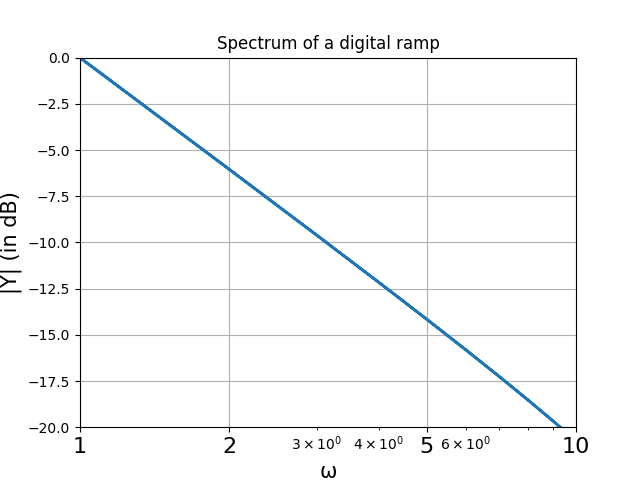
\includegraphics[scale=0.6]{Figure_4.png}
\caption{Computing circular convolution using linear convolution}
\label{fig:universe}
\end{figure}


\subsection{Question 7}
We now examine the Zadoff Chu Sequence. The Sequence has the following properties:

\begin{itemize}
\item It is a complex sequence.
\itemIt is a constant amplitude sequence.
\item The auto correlation of a Zadoff–Chu sequence with a cyclically shifted version of itself is zero.
\item Correlation of Zadoff–Chu sequence with the delayed version of itself will give a peak at that delay.t
\end{itemize}
The output obtained for correlation with a shifted version of itself was completely in line with these properties Given above.
\begin{alltt}
file2 = "x1.csv"

lines1 = []
with open(file2, 'r') as f2:
    csvreader = csv.reader(f2)
    for row in csvreader:
        lines1.append(row)

lines2 = []
for line in lines1:
    line = list(line[0])
    try :
        line[line.index('i')] = 'j'
        lines2.append(line)
    except ValueError:
        lines2.append(line)
        continue
x = [complex(''.join(line)) for line in lines2]
X = np.fft.fft(x)
x2 = np.roll(x, 5)
cor = np.fft.ifftshift(np.correlate(x2, x, 'full'))
print("The length of correlation array of x1 and shifted version of x1: ", len(cor))

figure()
xlim(0, 20)
make_graph(linspace(0, len(cor) - 1, len(cor)), abs(cor), 't →', 'Correlation →', 'Q7:
Auto-Correlation of x1 and shifted version(right shift by 5) of x1', 
"Ass10_Figure_6.png"),show()
\end{alltt}

\begin{figure}[h!]
\centering
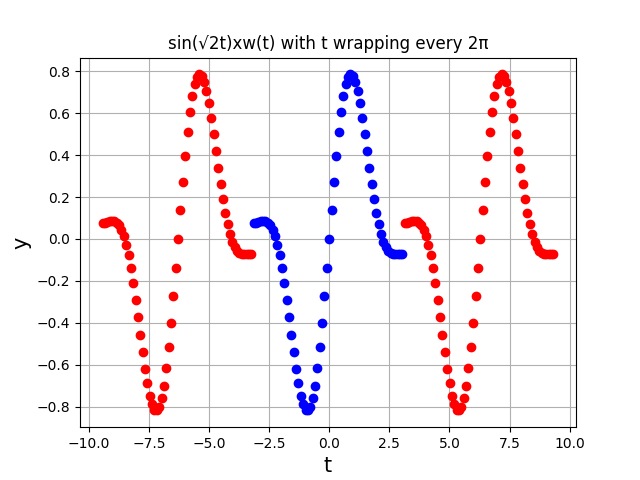
\includegraphics[scale=0.6]{Figure_5.png}
\caption{Correlation between Zadoff Chu Sequence and a shifted version of Zadoff chu sequence}
\label{fig:universe}
\end{figure}

\newpage
\section{Conclusion}
In this assignment we have explored different algorithms for convolution. We explored Linear convolution, Circular convolution and a hybrid between the two. After that we verified the properties of the given Zadoff-Chu Sequence using correlations. 


\end{document}